\chapter{Testy systemu (AK i JC)}
\label{cha:tests}

% setup
\graphicspath{{6_tests/static/}}

% content
Niniejszy rozdział stanowi szczegółowy raport z przeprowadzanych w środowisku docelowym testów systemu GGSS. Został on podzielony na trzy części, opisujące różne rodzaje przeprowadzanych przez autorów sprawdzeń. Pierwsza z nich przybliża informacje dotyczące przeprowadzanych w sposób cykliczny testów - nacisk położony został tutaj przede wszystkim na opis powtarzanej w każdej iteracji procedury pozwalającej zweryfikować poprawność działania systemu. Druga część stanowi opis sprawdzeń wykonywanych w czasie mającej miejsce w lipcu 2021 roku migracji systemu do nowego środowiska docelowego. Zamieszczone w niej informacje dotyczą wkładu autorów we wspomnianą migrację, obejmującego m.in. wykonanie testów warstwy sprzętowej systemu GGSS. Ostatnia część niniejszego rozdziału opisuje wykonane w sierpniu 2021 roku testy finalnej wersji projektu. W tym przypadku przedstawiony został szczegółowy raport, obejmujący weryfikację poprawności działania każdej wprowadzonej do systemu lub zmodyfikowanej funkcjonalności, badanie stabilności systemu ze względu na wykorzystywane zasoby oraz testy nowych elementów infrastruktury, takich jak skryptu zarządzające środowiskiem docelowym.

\section{Cykliczne testy systemu (AK)}
Praca nad projektem stanowiącym część dużego, rozwijanego przez wiele osób systemu wymaga, w celu zapewnienia poprawności działania, przeprowadzania cyklicznych testów w środowisku docelowym. Pozwala to na wczesne wykrywanie i eliminowanie pojawiających się w projekcie błędów. Regularne przeprowadzanie weryfikacji poprawności działania najnowszej wersji warstwy oprogramowania systemu GGSS pozwoliło ponadto na wygodne testowanie wprowadzanych przez autorów funkcjonalności - duża częstotliwość oznacza w tym przypadku możliwość testowania niewielkiego zbioru zmian.

Ze względu na fakt, iż autorzy pracują nad systemem GGSS od września 2019 roku, to procedura przeprowadzania tego typu testów zawarta została w manuskrypcie pracy inżynierskiej. Z tego też powodu nie został tutaj zamieszczony szczegółowy opis wykonywanych czynności. Elementem stanowiącym nowość względem procesu przeprowadzanego w ramach pracy inżynierskiej były testy wprowadzanych oraz modyfikowanych funkcjonalności. 

\clearpage
Na rysunku \ref{fig:tests_1} przedstawiony został stosowany przez autorów cykl pracy - kolorem niebieskim oznaczone zostały etapy związane z testowaniem systemu. Po przygotowaniu nowego wydania systemu autorzy rozpoczynali pierwszy etap testów, gdzie manualnej weryfikacji poddawane był nowe funkcjonalności oraz wprowadzone modyfikacje. Tego typu sprawdzenia wykonywane były zwykle za pomocą statycznie linkowanej wersji \emph{release} projektu. Jeśli tego typu testy zakończone zostały powodzeniem, następował drugi etap procesu testowania - trwajacy od kilku godzin do kilku dni test stabilności działania systemu, podczas którego moniotorowane były zapisywane w dzienniku zdarzeń inforacje oraz weryfikowane było zużycie zasobów. Opcjonalnie, jeśli testowane zmiany dotyczyły systemu budowania projektu, testom mogły zostać poddane inne jego wersje, np. \emph{debug}. Po zakończeniu tego etapu, jeśli nie zostały wykryte żadne błędy, system pozostawiany był w środowisku docelowym i traktowany jako wydanie stabilne. W przypadku niepowodzenia autorzy mieli możliwość wykonywania we wspomnianym środowisku dodatkowych sprawdzeń mających na celu ustalenie przyczyny błędu.

\begin{figure}[H]
\centering
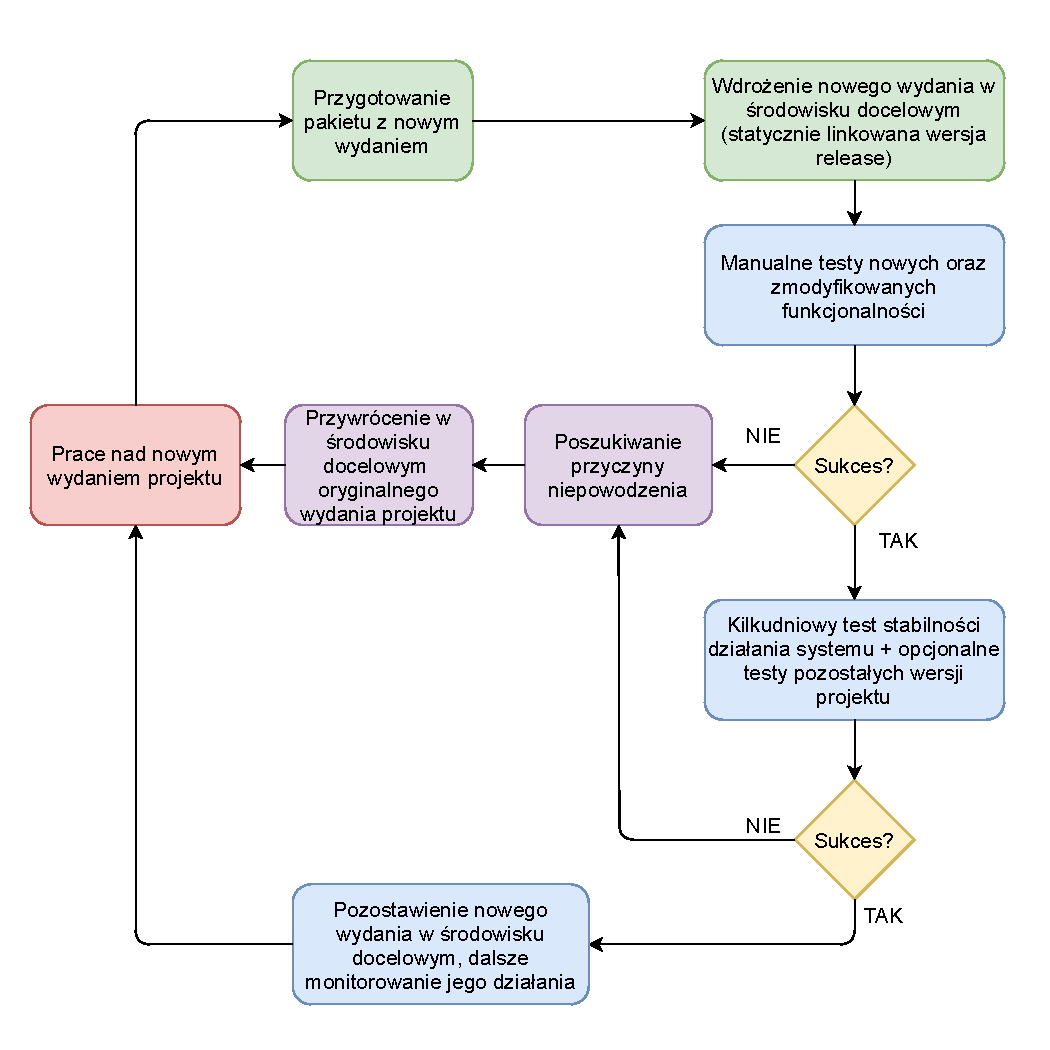
\includegraphics[width=0.85\textwidth]{algorithm.pdf}
\caption{Diagram przedstawiający stosowany przez autorów cykl pracy - kolorem niebieskim oznaczone zostały etapy związane z regularnymi testami oprogramowania.}
\label{fig:tests_1}
\end{figure}

\section{Testy po migracji systemu (JC)}

Jednym z ważniejszych etapów pracy magisterskiej była migracja całego systemu GGSS wraz ze sprzętem elektronicznym do nowego środowiska uruchomieniowego. Polegała ona na przeniesieniu kopii oprogramowania na nowy komputer oraz podłączeniu do niego wykorzystywanych urządzeń.

Cała operacja miała odbywać się w ramach wyjazdu autorów do CERN, natomiast ze względów pandemicznych wyjazd ten został ostatecznie odwołany. Z tego powodu migracja mogła zostać jedynie częściowo przeprowadzana przez autorów, znaczną część pracy wykonali natomiast eksperci, którzy znajdowali się na miejscu. W ramach migracji podłączyli oni sprzęt oraz przenieśli zawartość dysków ze starego komputera do nowej maszyny. Przed uruchomieniem całego systemu autorzy zdalnie zweryfikowali poprawność całego procesu. W ramach tego etapu wykorzystane zostały aplikacje do testowania sprzętu opisane w sekcji \ref{ch:hardware_testing}. W trakcie wykonywania testów sprzętu okazało się, że jedynie urządzenie połączone bezpośrednio do komputera jest wykrywane, a urządzenia połączone za pomocą hub'u USB nie. Rozwiązaniem problemu było podłączenie dodatkowego zasilania wymaganego przez wcześniej wspomniany hub. Upewniwszy się iż sprzęt podłączony jest poprawnie i jego działanie nie budzi zastrzeżeń, autorzy wykonali sprawdzenia pozostałych elementów środowiska, czyli: zainstalowanych bibliotek, wpisów w tabeli programu \lstinline{crontab} oraz poprawności umieszczenia plików projektu.

Po sprawdzeniu wszystkich wymaganych elementów środowiska autorzy rozpoczęli proces uruchamiania projektu GGSS wraz z jego główną aplikacją. W jego trakcie dokładnie monitorowano zachowanie warstwy oprogramowania oraz urządzeń elektronicznych. Oprócz zachowania aplikacji sprawdzane było również zużycie zasobów oraz ewentualne błędy, które mogły wystąpić ze względu na migrację. Po uruchomieniu projektu monitorowano jego działanie przez kilka godzin, a następnego dnia dokonano sprawdzenia dziennika zdarzeń. Nie stwierdzono żadnych problemów z systemem, a całość działała poprawnie. Migracja została uznana za zakończoną z sukcesem.

\section{Testy wersji finalnej (AK i JC)}
Niniejsza sekcja stanowi opis testów finalnej wersji systemu GGSS wykonanych w sierpniu 2021 roku. Sprawdzeniu poddane zostały zarówno wszystkie najważniejsze funkcjonalności systemu, jak również elementy infrastruktury projektu oraz wprowadzone przez autorów zmiany. Ponadto zbadane zostało zużycie zasobów systemu, takich jak pamięć, podczas długotrwałego, nieprzerwanego działania aplikacji \emph{ggss-runner}. 

\subsection{Testy funkcjonalności głównej aplikacji}
Autorzy dokonali szczegółowego sprawdzenia wszystkich przygotowanych modyfikacji i rozszerzeń. Ponadto testowane były elementy wchodzące w skład projektu od początku jego działania. W kolejnych akapitach opisane zostały poszczególne scenariusze testowe wraz z otrzymanymi przez autorów wynikami.

\subsubsection*{Działanie komend dedykowanych zasilaczom wysokiego napięcia}
Testom poddana została przygotowana przez autorów składnia komend służących do komunikacji z zasilaczami wysokiego napięcia. Wykonane zostały sprawdzenia wszystkich trzech typów poleceń (MON, SET, RAW) przy zastosowaniu zróżnicowanych konfiguracji opisujących moduły, kanały oraz parametry. Listing \ref{lst:test_hw_1} przedstawia wyniki przykładowych trzech zapytań - we wszystkich przypadkach są one zgodne z oczekiwaniami. Ze względu na powtarzalny charakter sprawdzeń, nie zostały tutaj przytoczone wszystkie testowane scenariusze. Sprawdzona została ponadto obsługa błędów, wynikających m.in. z niepoprawnego formatu i zawartości przesyłanych poleceń. Biblioteka dokonuje poprawnej obsługi tego typu sytuacji.

\lstinputlisting[
    language=Cmd, 
    caption={Przykładowe wyniki działania komend służących do komunikacji z zasilaczami wysokiego napięcia. Otrzymane rezultaty są zgodne z oczekiwaniami.}, 
    label={lst:test_hw_1}
]{6_tests/code_samples/dim_hw_ok.txt}

\subsubsection*{Opróżnianie bufora urządzenia MCA}
Sprawdzone zostało poprawne wykonanie algorytmu pozwalającego na zapobieganie przepełnieniu bufora urządzenia MCA poprzez cykliczne przenoszenie jego zawartości do pamięci RAM komputera. 

% Ponieważ funkcjonalność ta jest opcjonalna, działanie systemu zweryfikowane zostało w obu możliwych przypadkach funkcjonowania. Sprawdzeniu zostały poddane zar

% Kolejne testy dotyczyły funkcjonalności pozwalającej na zapobieganie przepełnieniu bufora urządzenia MCA. W tym przypadku sprawdzone zostały scenariusze takie jak: działanie programu, gdy w pliku konfiguracyjnym nie została wyspecyfikowana wartość parametru \lstinline{mcaRefreshInterval}, dzialanie gdy taki parametr w pliku został określony oraz wykonywanie pomiarów o zróżnicowanym czasie trwania. Testy tej funkcjonalności zakończyły się powodzeniem ...

\subsubsection*{Działanie algorytmu dopasowującego funkcję do zebranych danych}


\subsubsection*{Działanie komend sterujących systemem GGSS}


\subsubsection*{Pozostałe testy}
% zmiana wszystkich parametrow
%





\clearpage
\subsection{Testy aplikacji oraz skryptów do obsługi sprzętu fizycznego}

W ramach testów wersji finalnej przeprowadzono sprawdzenie wszystkich aplikacji do obsługi sprzętu fizycznego, które były modyfikowane, czy też utworzone od zera przez autorów. Teste były przeprowadzane w środowisku produkcyjnym przy wyłączonym systemie ggss, a dokładnie z wyłączoną główną aplikacją projektu. W celu sprawdzenia poprawności działania oraz funkcjonalności wykonano zaówno komendy z użyciem trybu interaktywnego utworzonych aplikacji, jak i trybu scenariuszowego. W pierwszej kolejności testom została poddana aplikacja odpowiedzialna za obsługę zasilacza wysokiego napięcia, czyli \emph{high-voltage-service-app}. Listing \ref{lst:high-voltage-service-app-startup} przedstawia wywołanie aplikacji z wszystkimi wymaganymi argumentami oraz wiadomość powitalną aplikacji. W ramach tejże wiadomości otrzymujemy informację o utworzeniu połączenia z modułem zasilacza, a dokładniej o dodaniu danego modułu do repozytorium. Następnie wyświetlana jest informacja o wykorzystaniu truby interaktywnego wraz z krótką pomocą zawierającą format komend.

\begin{lstlisting}[language=cmd,caption={Uruchomienie aplikacji \emph{high-voltage-service-app} w trybie interaktywnym},label={lst:high-voltage-service-app-startup},frame=single]
[jcierpic@pcatltrt02 high-voltage-service-app]$ ./high-voltage-app --dev-port=/dev/ggss_hv_0 --dev-modules 3
Connecting to HV using port /dev/ggss_hv_0 ...
Adding: /dev/ggss_hv_0:0 (alias:module0) to repository
Adding: /dev/ggss_hv_0:1 (alias:module1) to repository
Adding: /dev/ggss_hv_0:2 (alias:module2) to repository
Entering interactive mode ...
========================================
Usage:
<module_alias> - moduleX, where X is between 0 and given --dev-modules exclusive
hv <module_alias>:<channel_number> mon <param[,other_params]> - mon channel command
hv <module_alias> mon <param> - mon module command
hv <module_alias>:<channel> set <param> <value> - set channel command
hv <module_alias> raw <command_content> - raw command
help - print help message
quit - exit testing app
========================================
\end{lstlisting}

Listing \ref{lst:high-voltage-service-app-commands} zawiera przykład działania komend pozwalających na ustawienie wartości zasilania na wyjściu zasilacza, oraz pobrania tejże wartości wraz z asercją mającą na celu automatyczne sprawdzenie, czy oczekiwana wartość zgadza się z rzeczywistą. Trzecie wywołanie komendy ma za zadania sprawdzenie, czy w przypadku nieotrzymania zadanej wartości aplikacja poprawnie zgłosi błąd. Ostatnie z wywołań sprawdza, czy działająca jest funkcjonalność asercji z toleracją.

\begin{lstlisting}[language=cmd,caption={Komendy wykonywane w trybie interaktywnym aplikacji \emph{high-voltage-service-app}},label={lst:high-voltage-service-app-commands},frame=single]
>> hv module0:0 set vset 0
>>hv module0:0 set vset 0
<<OK: module0:0:VSET:OK;

>> assert hv module0:0 mon vmon 0
>>hv module0:0 mon vmon
<<OK: module0:0:VMON:0.0;
Assertion successful: target(0.000000) actual(0.000000)

>> assert hv module0:0 mon vmon 1
>>hv module0:0 mon vmon
<<OK: module0:0:VMON:0.0;
Error: Assertion failed: target(1.000000) actual(0.000000)

>> assertTol hv module0:0 mon vmon 2 10
>>hv module0:0 mon vmon
<<OK: module0:0:VMON:0.0;
Assertion with tolerance (10.000000) successful: target(2.000000) actual(0.000000)
\end{lstlisting}

Testom poddany został również tryb scenariuszowy, co przedstawia listing \ref{}. W przypadku trybu scenariuszowego zamiast informacji o możliwych do wykonania komendach otrzymujemy informacje o przetorzonych komendach z pliku scenriuszowego, które zostaną wykonane w trakcie działania zasadniczego. Następnie uruchamiane są wszystkie przetworzone scenariusze, których uruchomienia zażądał użytkownik.

\begin{lstlisting}[language=cmd,caption={Uruchomienie aplikacji \emph{high-voltage-service-app} w trybie scenariuszowym},label={lst:high-voltage-service-app-commands},frame=single]
[jcierpic@pcatltrt02 high-voltage-service-app]$ ./high-voltage-app --dev-port=/dev/ggss_hv_0 --dev-modules=3 --scenario-file=./sample_scenario.yml --scenarios=HighVoltageTestScenario
Connecting to HV using port /dev/ggss_hv_0 ...
Adding: /dev/ggss_hv_0:0 (alias:module0) to repository
Adding: /dev/ggss_hv_0:1 (alias:module1) to repository
Adding: /dev/ggss_hv_0:2 (alias:module2) to repository
Entering scenario mode ...
Parsing HighVoltageTestScenario HV scenario ...
Parsing hv module1:3 set vset 10.0 HV command ...
Parsing sleep 20000 HV command ...
Parsing assert hv module1:3 mon vset 10.0 HV command ...
Parsing assertTol hv module1:3 mon vmon 10.0 1.0 HV command ...
Parsing hv module1:3 set vset 0 HV command ...
Parsing sleep 20000 HV command ...
Parsing assert hv module1:3 mon vset 0 HV command ...
Parsing assert hv module1:3 mon vmon 0 HV command ...
Running HighVoltageTestScenario HV scenario ...
>>hv module1:3 set vset 10.0
<<OK: module1:3:VSET:OK;
>>hv module1:3 mon vset
<<OK: module1:3:VSET:10.0;
Assertion successful: target(10.000000) actual(10.000000)
>>hv module1:3 mon vmon
<<OK: module1:3:VMON:10.0;
Assertion with tolerance (1.000000) successful: target(10.000000) actual(10.000000)
>>hv module1:3 set vset 0
<<OK: module1:3:VSET:OK;
>>hv module1:3 mon vset
<<OK: module1:3:VSET:0.0;
Assertion successful: target(0.000000) actual(0.000000)
>>hv module1:3 mon vmon
<<OK: module1:3:VMON:0.0;
Assertion successful: target(0.000000) actual(0.000000)
\end{lstlisting}

Wszystkie testy aplikacji \emph{high-voltage-service-app} przebiegły pomyślne. Aplikacja wykonała wszystkie żądane czynności, a odpowiednie wartości pojawiły się na zasilaczu wysokiego napięcia. Zarówno tryb interaktywny, jak i scenariuszowy zostały uruchomione bez problemu. Aplikacja zachowywała się poprawnie również w przypadku, gdy oczekiwane było zgłoszenie błędu.

Następnie w podobny sposób przetestowane zostało dzianie aplikacji \emph{multiplexer-service-app}. Przetestowano zarówno jej tryb interaktywny, jak i scenariuszowy. Ze względu na to, że testy wyglądały analogicznie jak w przypadku aplikacji \emph{high-voltage-service-app}, a różnice stanowiły jedynie komendy oraz odpowiedzi od urządzenia, zaprezentowany został jedynie listing \ref{lst:multiplexer-service-app}, który przedstawia widomość powitalną aplikacji do obsługi multipleksera oraz kilka podstawowych komend.

\begin{lstlisting}[language=cmd,caption={Uruchomienie aplikacji \emph{high-voltage-service-app} w trybie scenariuszowym},label={lst:multiplexer-service-app},frame=single]
    [jcierpic@pcatltrt02 multiplexer-service-app]$ ./multiplexer-app --dev-port /dev/ttyUSB2
    Connecting to multiplexer using port /dev/ttyUSB2 ...
    Entering interactive mode ...
    ========================================
    Usage:
    getch - prints active channel
    setch <channel_number> - set new active channel
    getsn - prints MUX serial number
    setgetch <channel_number> - set new active channel and check it
    help - print help message
    quit - exit testing app
    ========================================
    >> getsn
    Printing MUX serial number ...
    Serial number: 260
    >> getch
    Trying to get active channel ...
    Active channel: 2
    >> setch 0
    Trying to set active channel ...
    Active channel set to 0
    >> getch
    Trying to get active channel ...
    Active channel: 0
    >> setgetch 2
    Trying to set active channel ...
    Active channel set to 2
    Trying to get active channel ...
    Success: active channel matches desired one
\end{lstlisting}

W przypadku aplikacji \emph{multiplexer-service-app} wszystkie testy udało się przeprowadzić pomyślnie. Nie stwierdzono żadnych błędów w działaniu wyżej wymienionej aplikacji. Wszystkie funkcjonalności, tryb interaktywny, jak i tryb scenariuszowy działały poprawnie.

Testy aplikacji \emph{high-voltage-killer} oraz skryptów składających się na system awaryjnego wyłączania zasilania wysokiego napięcia polegały na zarówno uruchomieniu samego programu i sprawdzeniu, czy jego działanie jest poprawne oraz na zasymulowaniu rzeczywistych warunków, w ramach których program powinien zostać uruchomiony.

W pierwszej kolejności wykorzystano wcześniej przetestowaną aplikację \emph{high-voltage-service-app} w celu ustawienia zasilania na zasilaczu wysokiego napięcia na wartość większą niż zero, następnie uruchomiono aplikację \emph{high-voltage-killer}, co przedstawia listing \ref{lst:high-voltage-killer}. W ramach działania aplikacja analizuje znajdujące się w systemie pliki urządzeń, następnie wybiera te, za pomocą których podłączone są zasilacze wysokiego napięcia. Następnie wykorzystując bibliotekę \emph{caenn1470-lib} zerowane są napięcia na wszystkich wyjściach wszystkich podłączonych modułów. Aplikacja prewencyjne próbuje zerować napięcia na modułach od 0 do 7, nawet, gdy tylko 3 moduły są uruchomione, natomiast komendy wysyłane są jedynie do podłączonych modułów.

\begin{lstlisting}[language=cmd,caption={Uruchomienie aplikacji \emph{high-voltage-killer}},label={lst:high-voltage-killer},frame=single]
[jcierpic@pcatltrt02 high-voltage-killer]$ ./high-voltage-killer
Running on port: /dev/ggss_hv_0
Killing voltage on: /dev/ggss_hv_0:0
Killing voltage on: /dev/ggss_hv_0:1
Killing voltage on: /dev/ggss_hv_0:2
Killing voltage on: /dev/ggss_hv_0:3
[ERROR] Device is not responding.
Killing voltage on: /dev/ggss_hv_0:4
[ERROR] Device is not responding.
Killing voltage on: /dev/ggss_hv_0:5
[ERROR] Device is not responding.
Killing voltage on: /dev/ggss_hv_0:6
[ERROR] Device is not responding.
Killing voltage on: /dev/ggss_hv_0:7
[ERROR] Device is not responding.
\end{lstlisting}

Następnie ponownie wykorzystując aplikację \emph{hgih-voltage-service-app} sprawdzono, czy rzeczywiście napięcie zostało wyzerowane. Wykonując odpowiednie komendy stwierdzono, że test przebiegł pomyślnie.

Oprócz samego działania aplikacji \emph{high-voltage-killer} przetestowano również funkcjonalności dostarczane w skryptach współpracujących z tą aplikacją:
\begin{itemize}
    \item Uruchomienie aplikacji \emph{high-voltage-killer} jeżeli główna aplikacja ggss przestała działać i nie została uruchomiona w przeciągu 5 minut
    \item Możliwość zablokowania systemu awaryjnego wyłączania zasilania poprzez utworzenie pliku blokady.
    \item Ciągłe działanie systemu awaryjnego wyłączania zasilania w przypadku braku pliku blokady.
    \item Awaryjne wyłączenie zasilania w przypadku otrzymania signału SIGTERM
\end{itemize}

Przeprowadzone testy wszystkich wyżej wymienionych funkcjonalności przebiegły pomyślnie. Nie napotkano żadnych przeszkód w trakcie ich wykonywania.
Dodatkowo przeprowadzaono testy aplikacji \emph{device-detector}, której zadaniem jest raportowanie informacji o podłączonych do systemu urządzeniach fizycznych, które wymagane są do działania systemu ggss. Również w tym przypadku proces przebiegł pomyślne. W celu osiągnięcią stu procentowej pewności, iż wszystkie aplikacje związane ze sprzętem fizycznym działają poprawnie w nowym środowisku testom została poddana również aplikacja \emph{mca-service-app}. Uruchomienie tejże aplikacji nie budziło żadnych problemów, a wyniki jej działania były poprawne. Wraz z zakończemiem tego testu wszystkie aplikacje oraz skrypty związane ze sprzętem zostały w pełni przetestowane, dzięki czemu autorzy mogli być pewni poprawności zaimplementowanych funkcjonalności.


\subsection{Testy zużycia zasobów}
% Względem pracy inżynierskiej autorzy dokonali zmian w wykorzystywanych do przeprowadzania testów narzędziach. Jednym z nich był skrypt pozwalający na monitorowanie zużycia zasobów przez aplikację 